\section{Auswertung}
\label{sec:Auswertung}

\subsection{Phänomenologische Beobachtungen des Supraleiters}
\label{sec:beo}
Zu Beginn des Versuches werden die gemachten Beobachtungen der verschiedenen
Magnet-Supraleiter-Anordnungen geschildert. In den drei folgenden Abbildungen
\ref{fig:SL1}, \ref{fig:SL2} und \ref{fig:SL3} ist gut zu erkennen,
wie der Magnet, bedingt durch den Meißner-Ochsenfeld-Effekt, eigenstabil über dem
Supraleiter schwebt. Dabei rotiert in Abbildung \ref{fig:SL1} ein kleiner Magnet
\#M1 in einer schrägen Position über dem SL \#2 Supraleiter um seine Achse hin und zurück.
Hingegen rotiert, relativ zu seiner Achse, der größere Magnet \#M2 in Abbildung \ref{fig:SL2}
parallel zum SL \#3 Supraleiter hin und zurück.

\begin{figure}[H]
\centering
	\begin{subfigure}[t]{0.45\textwidth}
    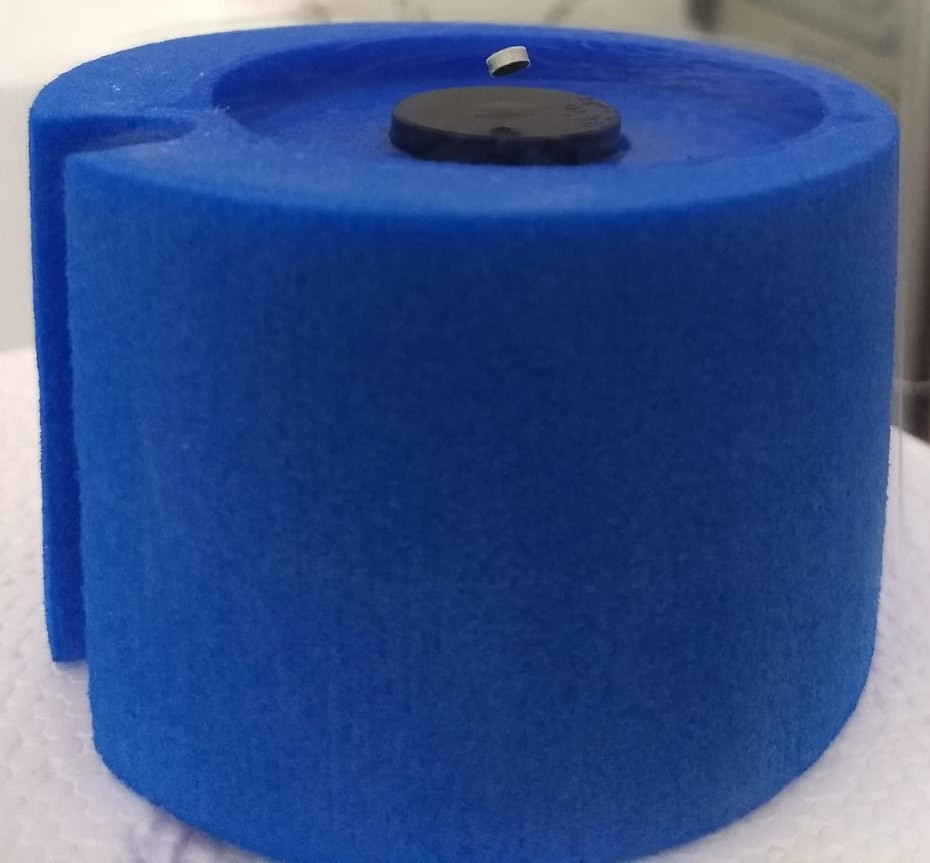
\includegraphics[width=\textwidth]{Auswertung/SL_1.jpg}
    \caption{Der SL \#2 Supraleiter zusammen mit einem \#M1 Permanentmagnet auf einem Styroporbehältnis
    mit flüssig Stickstoff.}
    \label{fig:SL1}
	\end{subfigure}
	~
	\begin{subfigure}[t]{0.45\textwidth}
    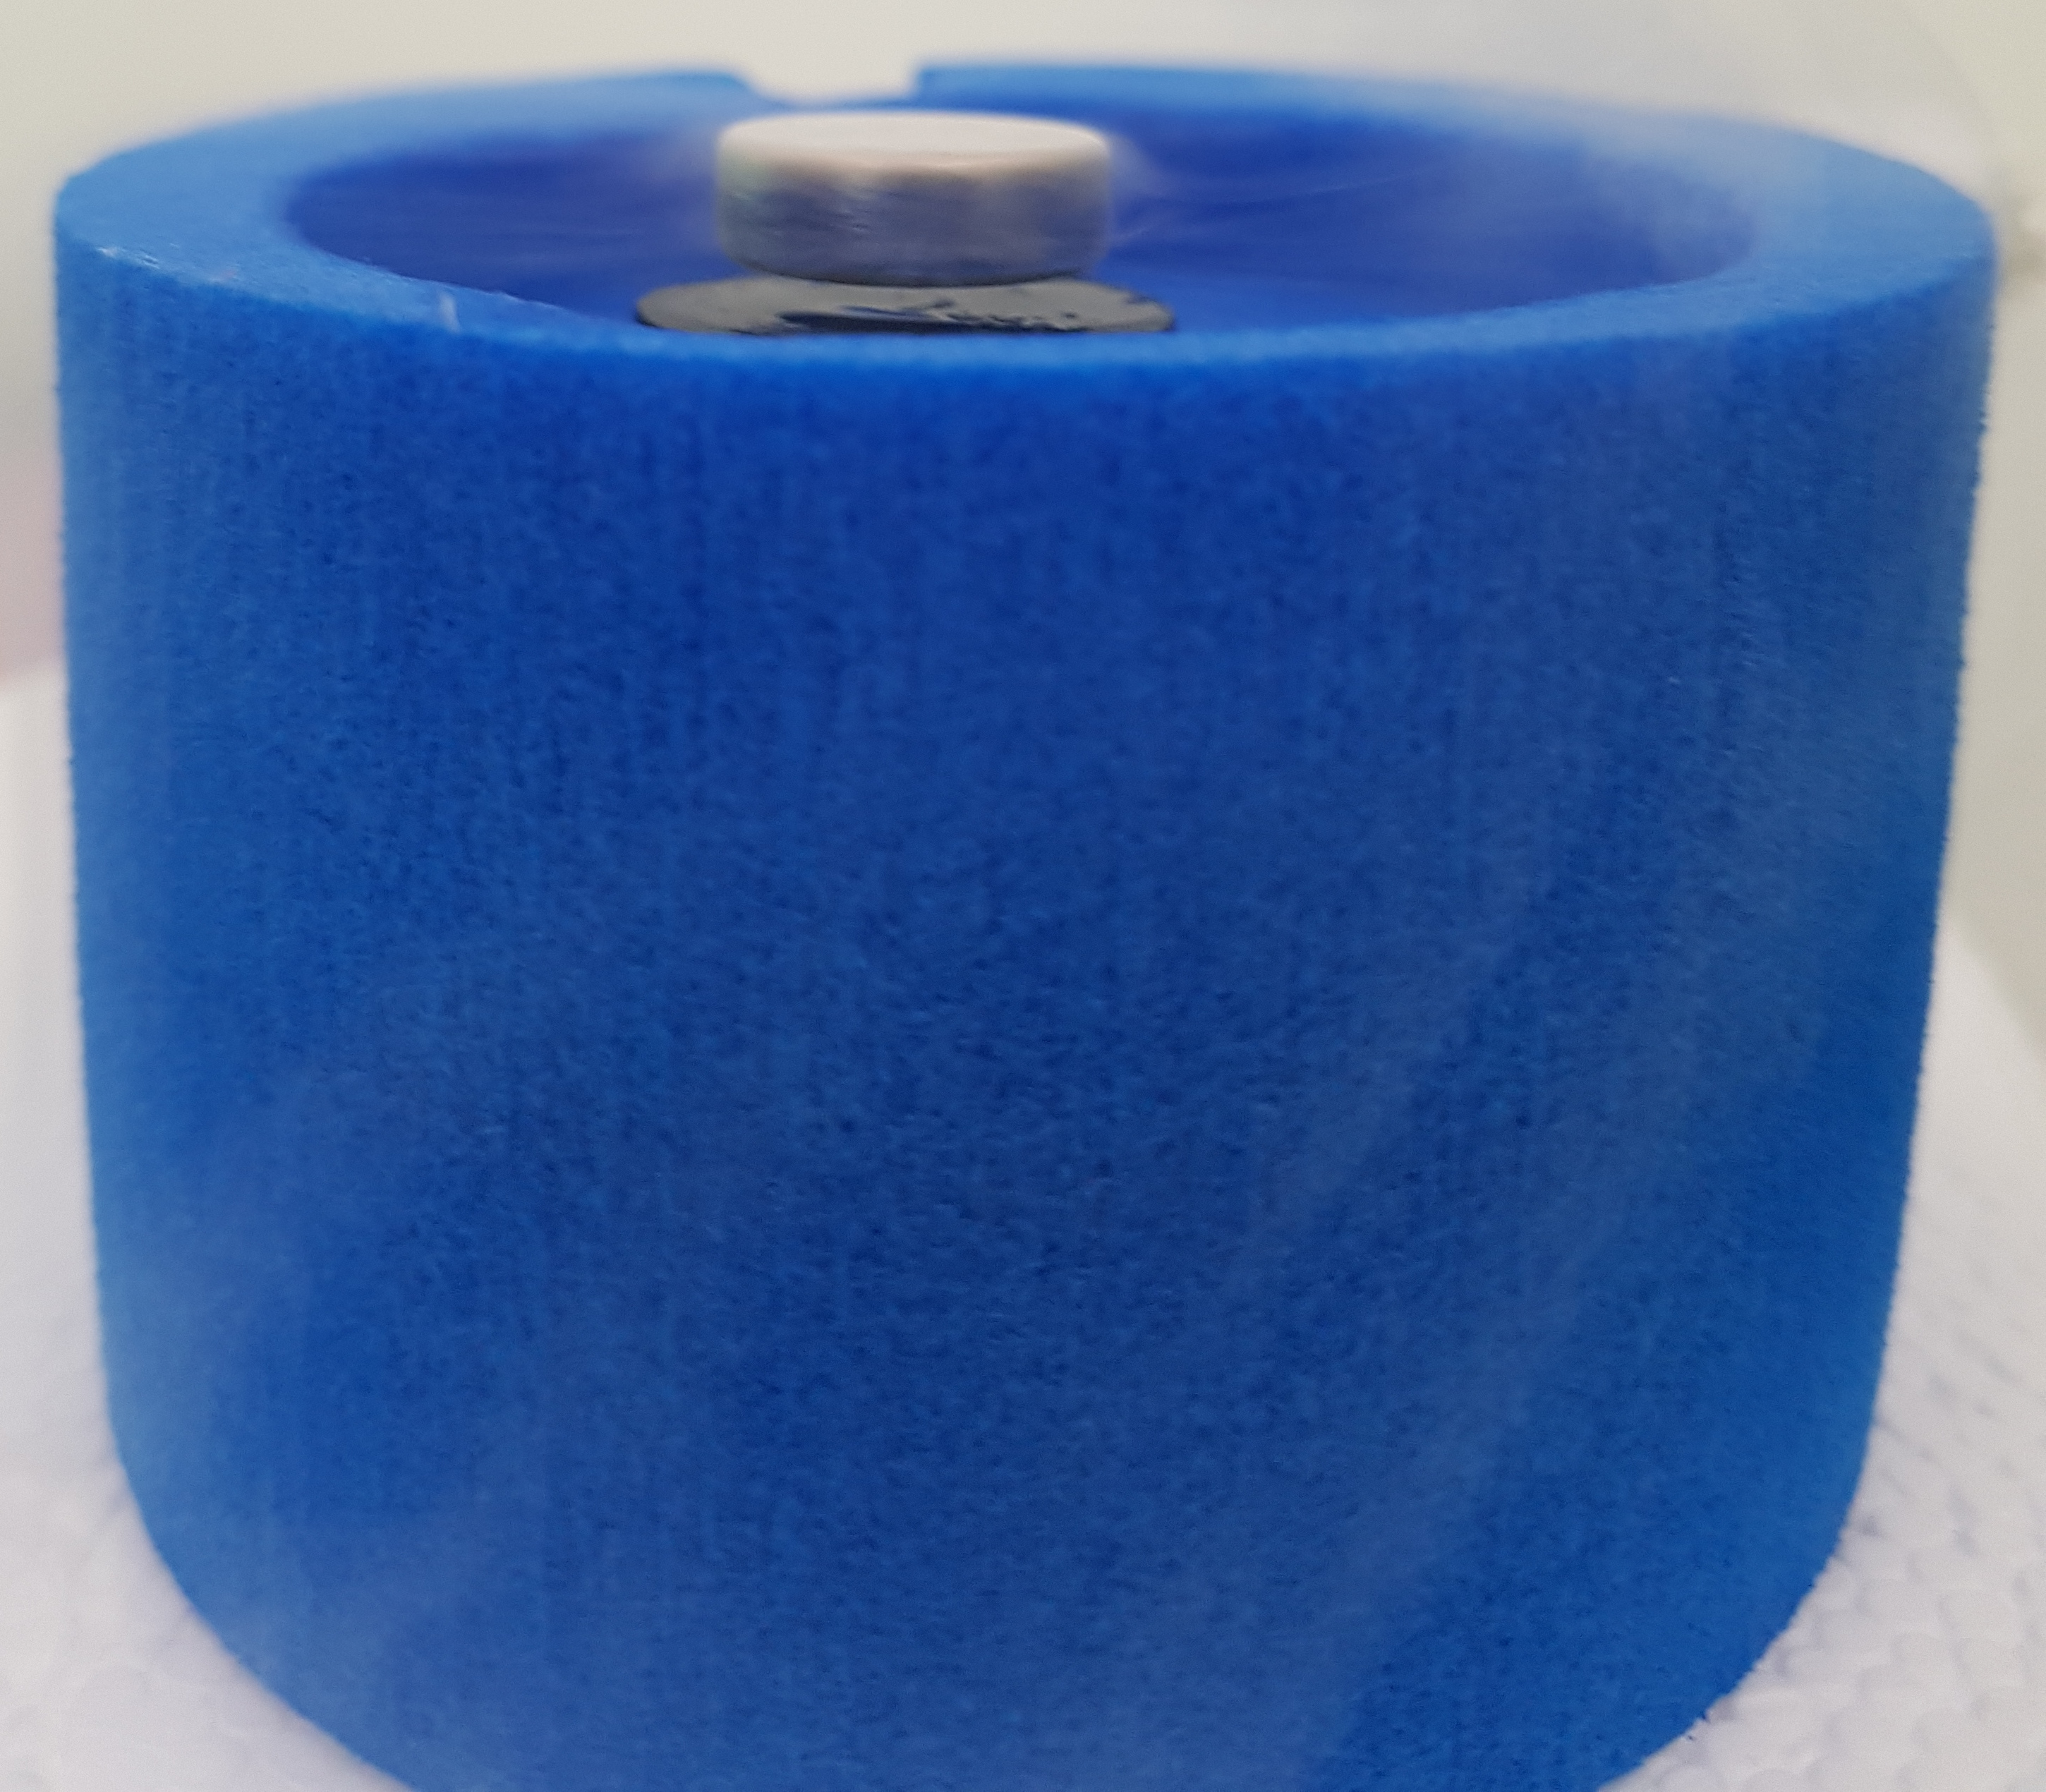
\includegraphics[width=1.06\textwidth]{Auswertung/SL_2.jpg}
    \caption{Der SL \#3 Supraleiter zusammen mit dem \#M2 Permanentmagnet auf einem Styroporbehältnis
    mit flüssig Stickstoff.}
    \label{fig:SL2}
	\end{subfigure}
\end{figure}

\noindent
Besonders attraktiv sind diese Eigenschaft in der Technik,
da so eine berührungslose Kraftübertragung realisiert werden kann. So lassen sich
beispielsweise supraleitende Magnetlager wie in Abbildung \ref{fig:SL3} realisieren.
In Abbildung \ref{fig:SL3} ist dazu ein Pinning-Stab zusammen mit dem \#M2
Permanentmagneten zu sehen. Diese Konfiguration schwebt über dem SL \# 3 Supraleiter.
Wird dem Pinning-Stab samt \#M2 Magnet ein Impuls übertragen, so rotiert die Konfiguration
stabil über dem SL \#3 Supraleiter. Wird die Anordnung aus Abbildung \ref{fig:SL3} nun
am Pinning-Stab angehoben, so bleibt die Konstellation bestehen. Der SL \# 3 Supraleiter
schwebt nun unter dem Magneten, dieser Effekt wird der Suspension zugeschrieben.
Sind die Pinning-Kräfte stark genug, so lassen sich Rotationsbewegungen in
sämtliche Raumrichtungen ermöglichen (siehe Abbildung \ref{fig:SL4}).

\begin{figure}[H]
\centering
	\begin{subfigure}[t]{0.45\textwidth}
    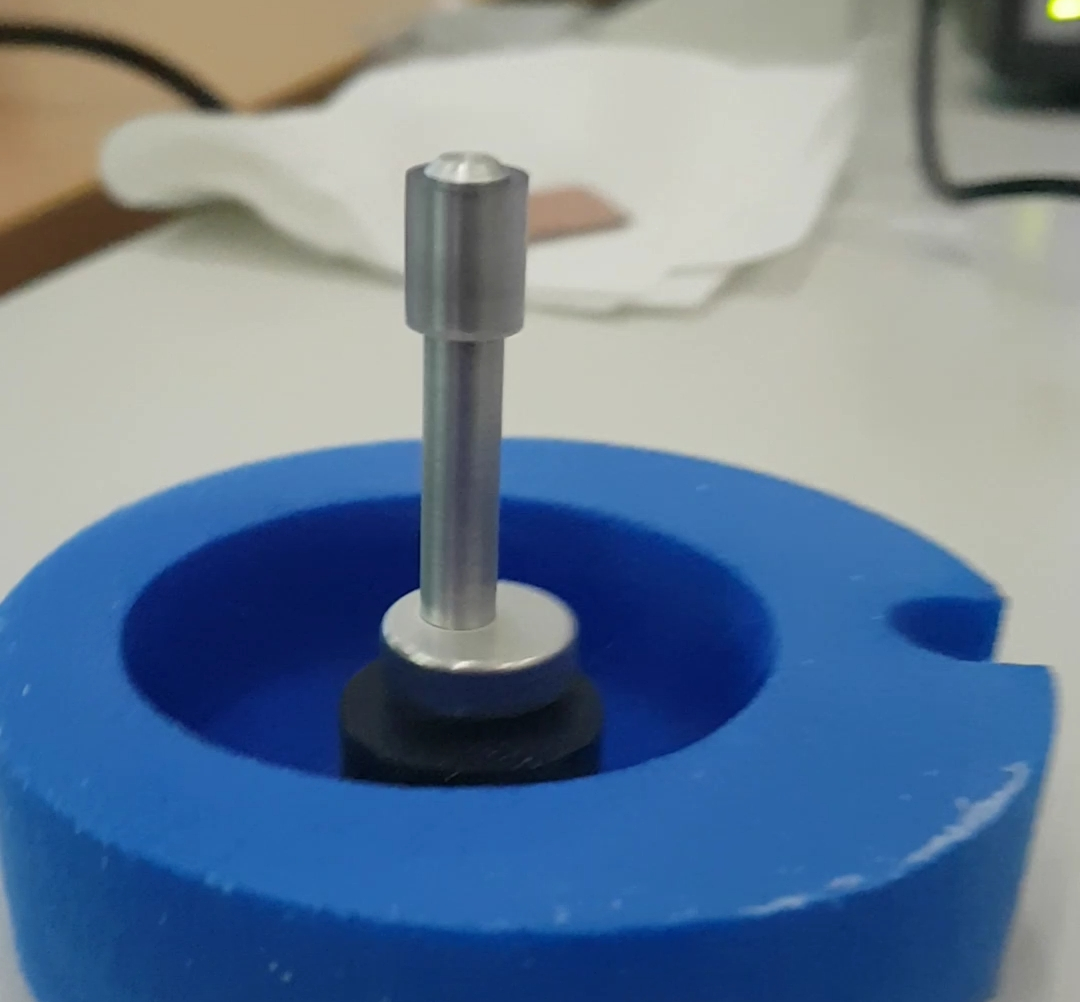
\includegraphics[width=\textwidth]{Auswertung/SL_3.jpg}
    \caption{Magnetlager aus dem SL \#3 Supraleiter zusammen mit einem
    \#M2 Permanentmagnet und einem Pinning-Stab auf einem Styroporbehältnis mit
    flüssig Stickstoff.}
    \label{fig:SL3}
	\end{subfigure}
	~
	\begin{subfigure}[t]{0.45\textwidth}
    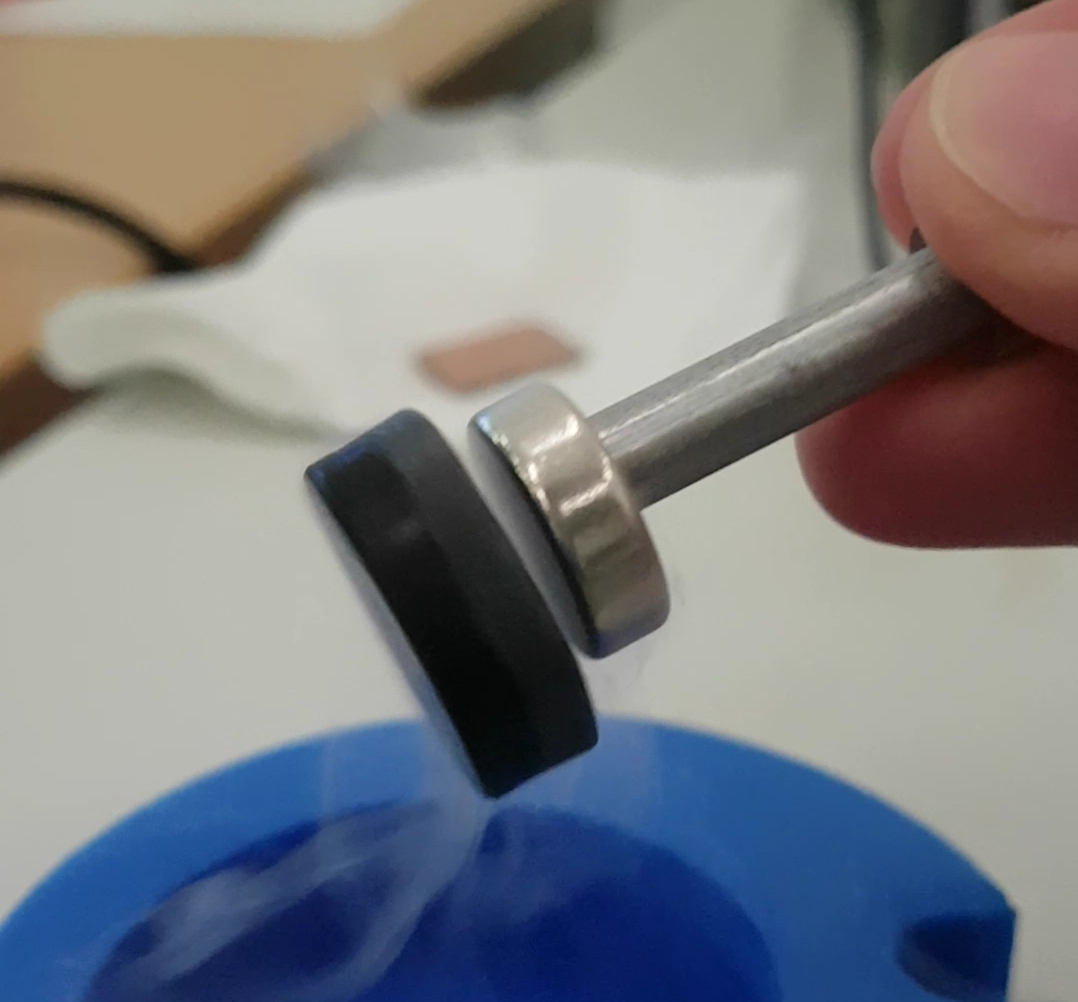
\includegraphics[width=\textwidth]{Auswertung/SL_4.jpg}
    \caption{Magnetlager aus dem SL \#3 Supraleiter zusammen mit einem
    \#M2 Permanentmagnet und einem Pinning-Stab in einer Schräglage angehoben.}
    \label{fig:SL4}
	\end{subfigure}
\end{figure}

\subsection{Bestimmung der kritschen Temperatur $T_{\text{c}}$ via Meißner-Ochsenfeld-Effekt}
\label{sec:TcOchse}

Um die Spannung $U_{\text{TS,Si}}$ am Silizium-Temperatursensor in Temperatur $T$
umzurechnen, wird ein Polynom vierten Grades genutz:

\begin{equation*}
  T(U_{\text{TS,Si}}) = a_0 + a_1 \cdot U_{\text{TS,Si}} + a_2 \cdot U_{\text{TS,Si}}^2
  + a_3 \cdot U_{\text{TS,Si}}^3 + a_4 \cdot U_{\text{TS,Si}}^4
  \label{FA1}
\end{equation*}

\noindent
dabei sind die Kalibierungsdaten $a_{i}$ mit $i \in$ {0,..,4} dem Datenblatt
zu entnehmen. Das dabei resultierende Verhältnis zwischen Temperatur $T$ und der
Messzeit $t$ ist in Abbildung \ref{fig:TcOchse} dargestellt. Dabei wird die anfängliche
Messzeit abgeschnitten, bei der keine Temperaturänderung statt findet und ein
neuer zeitlicher Nullpunkt gesetzt. So lässt sich das Verhalten bei der
Temperaturerhöhung besser untersuchen. Der Zeitpunkt an dem der \#M1 Magnet wieder
auf dem Supraleiter aufliegt, ist jeweils mit einem gelben Kreis gekennzeichnet.
Alle drei Messungen zeigen anfangs einen starken Temperaturanstieg. Etwa $\SI{4}{second}$
nachdem die jeweilige kritsche Temperatur $T^{\text{MCE}}_{\text{c}}$ erreicht ist, zeigen
Messung 1 und 2 ein schwächer werdenden Temperaturanstieg, bis dieser sich nach
weiteren $\SI{5}{\second}$ annähernd linear verhält. Messung 3 hingegen, zeigt
sofort nachdem die kritische Temperatur $T^{\text{MCE}}_{\text{c}}$ erreicht ist, ein linearen
Zuwachs der Temperatur.\\
Die sich dabei ergebende kritsche Temperatur $T^{\text{MCE}}_{\text{c}}$ der einzelnen
Messungen ist in Tabelle \ref{tab:TcOchse} aufgelistet. Die Abschätzung des
systematischen Fehlers von $\SI{5}{\kelvin}$ ergibt sich teils daraus, dass das
Absenken des \#M1 Magnets nicht abrupt passiert, sondern in einem gewissen Messbereich.
Auch spielt die Position des Temperatursensors eine Rolle. Denn dieser liegt
möglicherweise nicht optimal auf dem SL \#2 Supraleiter auf. Ein Temperaturgradient
am SL \#2 Supraleiter, welcher die Messung verfälschen würde, ist ebenfalls nicht
auszuschließen. Da der Temperatursensor im Werk kalibriert wurde, wird der Fehler
beim Messen eher als gering eingeschätzt.
Durch Mittelung der kritschen Temperaturen $T^{\text{MCE}}_{\text{c}}$ der einzelnen Messungen
ergibt sich $\bar{T}^{MCE}_{\text{c}}$, mit dem Fehler $\Delta \bar{T}^{MCE}_{\text{c}} =
\Delta T^{MCE}_{\text{c}}/\sqrt{3}$.



\begin{figure}[H]
    \centering
    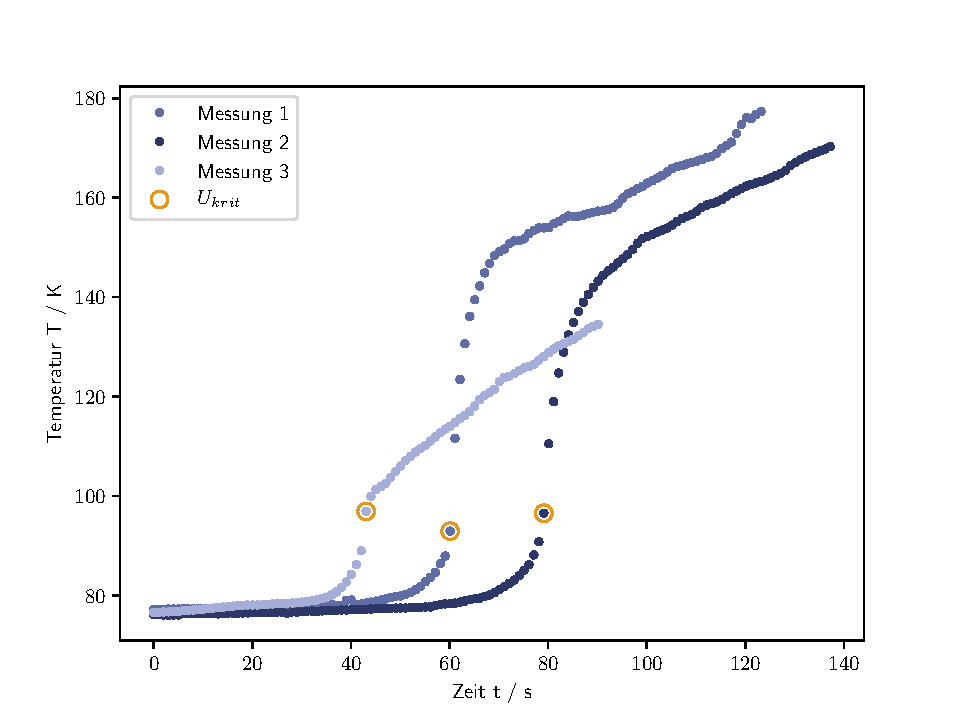
\includegraphics[width=0.8\textwidth]{Auswertung/T_krit_Si/T_krit.pdf}
    \caption{Bestimmung der kritschen Temperatur anhand von drei Messungen mittels
    des Meißner-Ochsenfeld-Effekts. Die gelben Kreise kennzeichnen den Zeitpunkt,
    an dem der \#M1 Magnet wieder auf dem SL \#2 Supraleiter aufliegt. Es werden
		allen Messwerten einen systematischen Fehler von $\SI{\pm5}{\kelvin}$
		zugeschrieben.}
    \label{fig:TcOchse}
\end{figure}

\begin{table}
  \centering
  \caption{Kritsche Temperatur $T^{\text{MCE}}_{\text{c}}$ für drei Messungen.}
  \label{tab:TcOchse}
  \sisetup{table-format=1.2}
  \begin{tabular}{S S S | S}
    \toprule
    \multicolumn{3}{c}{$T^{\text{MCE}}_{\text{c}}$ / K} & {$\bar{T}^{\text{MCE}}_{\text{c}}$ / K} \\
    {Messung 1} & {Messung 2} & {Messung 3} & {Mittel} \\
    \midrule
    {92,93\pm5} & {96,53\pm5} & {96,90\pm5} & {95,45\pm2,89} \\
    \bottomrule
  \end{tabular}
\end{table}


\subsection{Bestimmung der kritschen Temperatur $T_{\text{c}}$ via 4-Punkt-Messung}
\label{sec:Tc4punkt}
Im folgendem wird im Unterkapitel \ref{sec:ohneB} der SL \#1 Supraleiter ohne
Störung eines Magnetfeldes untersucht und damit die kritsche Temperatur
$T^{\text{4PM}}_{\text{c}}$ bestimmt. Dann wird im Unterkapitel \ref{sec:mitB}
die Messung mit dem \#M3 Magneten für zwei verschiedenen Abstände wiederholt.\\
Der Platin-Sensor erlaubt es die Temperatur am SL \#1 Supraleiter zu bestimmen.
Dazu wird der gemessene Widerstand $R_{\text{TS,Pt}}$ durch ein Polynom dritten
Grades:

\begin{equation*}
  T(R_{\text{TS,Pt}}) = a_0 + a_1 \cdot R_{\text{TS,Pt}} + a_2 \cdot R_{\text{TS,Pt}}^2
  + a_3 \cdot R_{\text{TS,Pt}}^3
  \label{FA2}
\end{equation*}

\noindent
in Temperatur $T$ umgerechnet, wobei $a_{i}$ mit $i \in$ {0,..,3} dem
Datenblatt des Platin-Sensors entnommen wird. Der SL \#1 Supraleiter, sowie
der Platin-Sensor befinden sich in einem geschlossenem Plexiglasgehäuse, was
die Messung vor äußeren Einflüssen schützt. Allerdings kann sich beim auftauen
so besser Flüssigkeit ansammeln, welche das Messergebnis verfälschen können.
Der Platin-Sensor ist vom Werk aus kalibriert und arbeitet damit sehr genau.
Ein Temperaturgradient am Supraleiter zum Platin-Sensor ist auch hier nicht
auszuschließen. Der systematische Fehler wird damit auf $\SI{\pm2}{\kelvin}$
geschätzt. Zusätzlich wird ein Ablesefehler bei der Bestimmung der kritschen
Temperatur $T^{\text{4PM}}_{\text{c}}$ dazugeschätzt. Dieser bildet sich durch
die Mittelung von vier Temperaturänderungen $\Delta T^{\text{4PM}}_{i,i-1}
= |T^{\text{4PM}}_{i}-T^{\text{4PM}}_{i-1}|$
um die kritsche Temperatur $T^{\text{4PM}}_{\text{c}}$:

\begin{equation*}
	\Delta \bar{T}^{\text{4PM}}_{\text{c}} = \frac{
																								 \Delta T^{\text{4PM}}_{\text{c-1,c-2}}
																								+\Delta T^{\text{4PM}}_{\text{c,c-1}}
																								+\Delta T^{\text{4PM}}_{\text{c+1,c}}
																								+\Delta T^{\text{4PM}}_{\text{c+2,c+1}}
																								}
																								{4}
\label{FA3}
\end{equation*}

\noindent

\subsubsection{Ohne Magnet}
\label{sec:ohneB}

Das temperaturabhängige Verhalten des SL \#1 Supraleiter-Widerstandes $R_{\text{SL}}$,
ohne Störung durch einen Magnetfeld, bei einem Durchlaufstrom
$I$ von $\SI{0.6}{\ampere}$ ist in Abbildung \ref{fig:Tc4PM} dargestellt. Der
SL \#1 ist zwischen $\SI{76\pm2}{\kelvin}$ und etwa $\SI{117\pm2}{\kelvin}$ supraleitend,
denn hier zeigt sich ein Widerstandswerte von Null. Fehlerhaft gemessene negative
Widerstandswerte sind größtenteils
aus dem Ausschnitt skaliert, weshalb Lücken, wie z.B. zwischen $\SI{80\pm2}{\kelvin}$
und $\SI{90\pm2}{\kelvin}$, entstehen. Diese und weitere Sprungwerte (beispielsweise
zwischen $\SI{115\pm2}{\kelvin}$ und etwa $\SI{116\pm2}{\kelvin}$) sind Messfehler, welche
sich größtenteils nicht im interessante Bereich aufhalten. Der interessante Bereich
ist der, an dem der Widerstand $R_{\text{SL}}$ eine stetige Zunahme erfährt.
Bei einer Temperatur von etwa $\SI{117,36\pm2,60}{\kelvin}$ zeigt sich der erste
Widerstandsanstieg von $\SI{0,1}{\milli\ohm}$. Danach ist der Widerstandszuwachs
sehr stark, bis dieser sich bei etwa $\SI{125\pm2}{\kelvin}$ annähernd linear
verhält.


\begin{figure}[H]
    \centering
    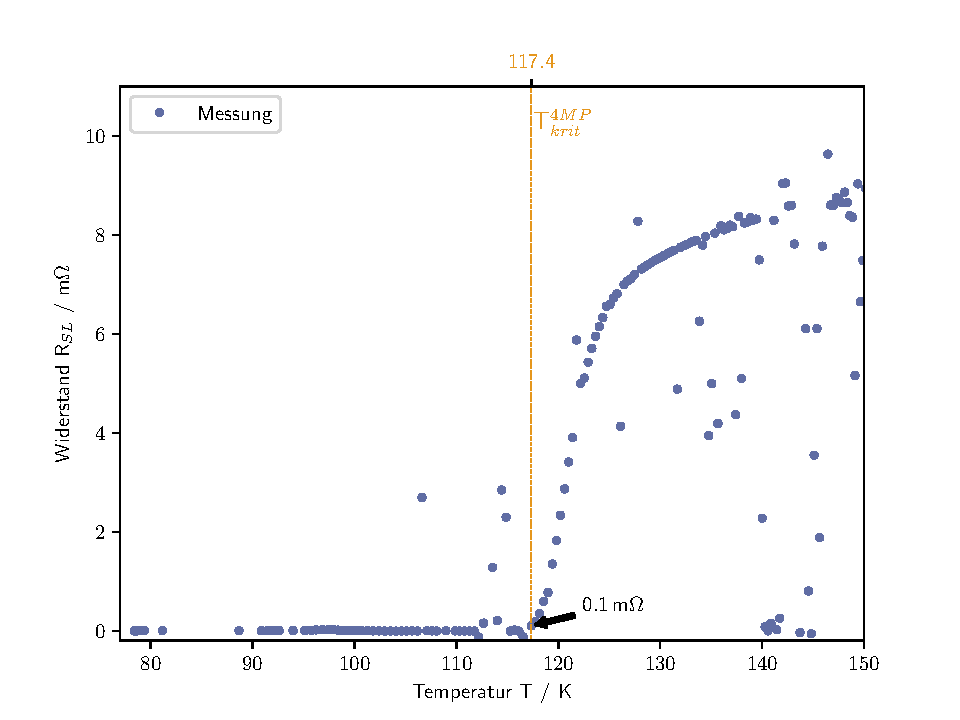
\includegraphics[width=0.8\textwidth]{Auswertung/T_krit_Pt/R_T.pdf}
    \caption{Bestimmung der kritschen Temperatur des SL \#1 Supraleiter ohne Magneten
		anhand einer 4-Punkt-Messung. Die Temperatur $T$ wird mit einem Platin-Sensor
		ermittel, wobei der Widerstand $R_{\text{SL}}$ bei einem Strom $I$ von $\SI{0.6}{\ampere}$
		gemessen wird. Die gelbe Markierung kennzeichnet die kritsche Temperatur
		$T^{\text{4PM}}_{\text{c}}$. Es werden allen Messwerten einen systematischen
		Fehler von $\SI{\pm2}{\kelvin}$	zugeschrieben.}
    \label{fig:Tc4PM}
\end{figure}

\subsubsection{Mit Magnet}
\label{sec:mitB}
Die Messung für einen Magnetabstand von $\SI{10}{\milli\meter}$ ist in Abbildung
\ref{fig:Tc4PM10}, und die in einem Abstand von $\SI{16}{\milli\meter}$ ist
in Abbildung \ref{fig:Tc4PM16} dargestellt. Beide sind ab $\SI{78\pm2}{\kelvin}$
bis zu kritschen Temperatur $T^{\text{4PM}}_{\text{c}}$ zunächst supraleitend.
Zuerst werden die beiden Abbildungen \ref{fig:Tc4PM10} und \ref{fig:Tc4PM16}
miteinander verglichen. Es fällt auf, dass die Messung aus Abbildung \ref{fig:Tc4PM10}
deutlich mehr Sprungwerte gemessen hat, als die Messung aus Abbildung \ref{fig:Tc4PM16}.
Damit ist in Abbildung \ref{fig:Tc4PM16} ein stetigerer Widerstandsanstieg zu erkennen.
Einige Sprungwerte sind in Abbildung \ref{fig:Tc4PM10} leider genau dort, wo der
Widerstandsanstieg anfängt. Dadurch lässt sich der anfängliche Widerstandszuwachs
erst bei $\SI{0.31}{\milli\ohm}$ bestimmen. Beide Messungen zeigen nach der kritschen
Temperatur $T^{\text{4PM}}_{\text{c}}$ einen ähnlich starken Widerstandsanstieg.
Werden beide Messungen (mit Magnet) mit der Messung aus Abbildung \ref{fig:Tc4PM}
(ohne Magnet) verglichen, fällt auf, dass der Widerstandsanstieg weniger stark ist.
In Tabelle \ref{tab:Tc4PM1016} sind die jeweilige kritschen Temperaturen
$T^{\text{4PM}}_{\text{c}}$ und die gemessene Magnetfeldstärke $B_{\text{ex}}$
aufgelistet. Gegen aller Erwartung, nimmt die $T^{\text{4PM}}_{\text{c}}$
bei einer größeren Magnetfeldstärke zu.


\begin{figure}[H]
    \centering
    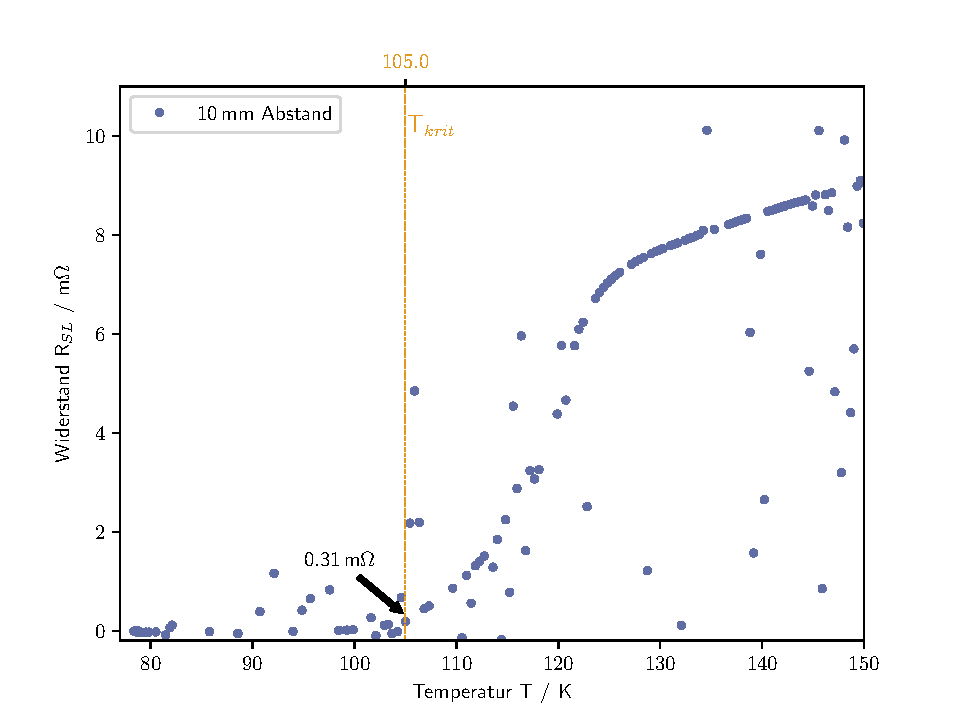
\includegraphics[width=0.8\textwidth]{Auswertung/T_krit_Pt/R_T_10mm.pdf}
    \caption{Bestimmung der kritschen Temperatur des SL \#1 Supraleiter mit dem
		\#M3 Magneten im Abstand von $\SI{10}{\milli\meter}$ anhand einer 4-Punkt-Messung.
		Die Temperatur $T$ wird mit einem Platin-Sensor	ermittel, wobei der Widerstand
		$R_{\text{SL}}$ bei einem Strom $I$ von $\SI{0.6}{\ampere}$ gemessen wird.
		Die gelbe Markierung kennzeichnet die kritsche Temperatur $T^{\text{4PM}}_{\text{c}}$.
		Es werden allen Messwerten einen systematischen Fehler von $\SI{\pm2}{\kelvin}$
		zugeschrieben.}
    \label{fig:Tc4PM10}
\end{figure}

\begin{figure}[H]
    \centering
    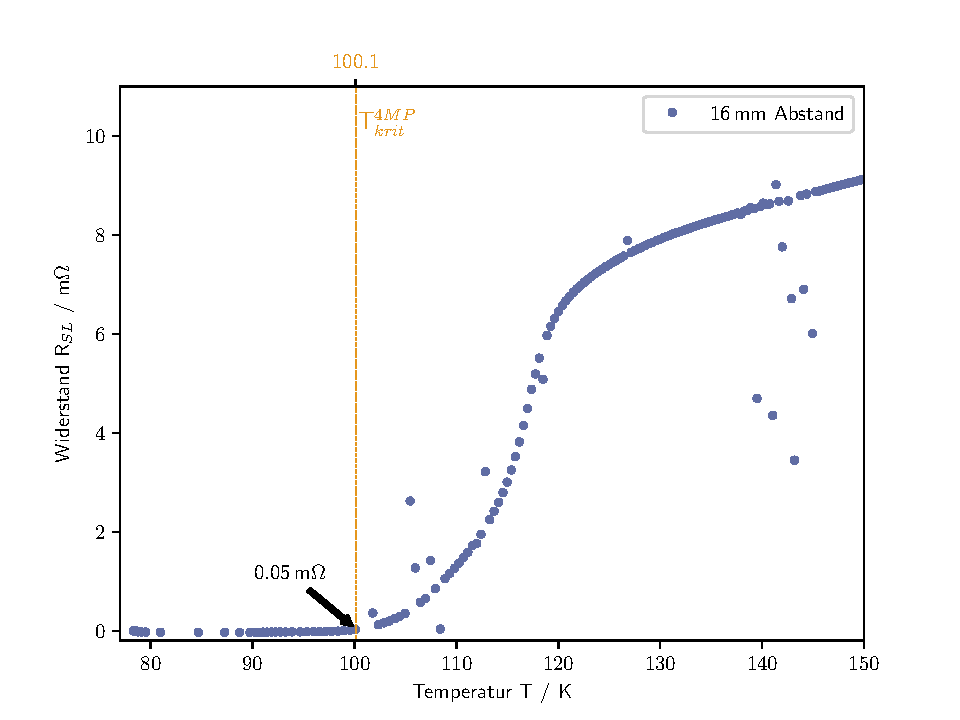
\includegraphics[width=0.8\textwidth]{Auswertung/T_krit_Pt/R_T_16mm.pdf}
    \caption{Bestimmung der kritschen Temperatur des SL \#1 Supraleiter mit dem
		\#M3 Magneten im Abstand von $\SI{16}{\milli\meter}$ anhand einer 4-Punkt-Messung.
		Die Temperatur $T$ wird mit einem Platin-Sensor	ermittel, wobei der Widerstand
		$R_{\text{SL}}$ bei einem Strom $I$ von $\SI{0.6}{\ampere}$ gemessen wird.
		Die gelbe Markierung kennzeichnet die kritsche Temperatur	$T^{\text{4PM}}_{\text{c}}$.
		Es werden allen Messwerten einen systematischen Fehler von $\SI{\pm2}{\kelvin}$
		zugeschrieben.}
    \label{fig:Tc4PM16}
\end{figure}

\begin{table}
  \centering
  \caption{Kritsche Temperatur $T^{\text{MCE}}_{\text{c}}$ für zwei
	unterschiedliche Magnetabstände.}
  \label{tab:Tc4PM1016}
  \sisetup{table-format=1.2}
  \begin{tabular}{S | S S}
    \toprule
    {Magnetabstand} & {kritsche Temperatur} & {Magnetfeldstärke} \\
    {d / mm} & {$T^{\text{MCE}}_{\text{c}}$ / K } & {$B_{\text{ex}}$ / mT} \\
    \midrule
    {10} & {105,01\pm2,63}	&	{142,7}	\\
		{16} & {100,12\pm2,86}	&	{23,5}	\\
    \bottomrule
  \end{tabular}
\end{table}

\subsection{Abschätzung der kritschen Stromstärke $I_{\text{c}}$}
\label{sec:Ic}
Im folgendem Unterkapitel \ref{sec:ohneB1} wird die kritsche Temperatur
$T^{\text{MCE}}_{\text{c}}$ bei einer 4-Punkt-Messung in Abhängigkeit von der
Durchlaufstromstärken $I$ untersucht. Die dabei entstehenden Fehler werden analog
zum Unterkapitel \ref{sec:Tc4punkt} abgeschätzt. Im zweiten Unterkapitel
\ref{sec:mitB1} wird die Messung mit Magnetfeld durchgeführt.

\subsubsection{Ohne Magnet}
\label{sec:ohneB1}
Eine 4-Punkt-Messung ohne Magnetfeld wird für jeweils fünf unterschiedlichen
Stromstärken ($I=\SI{0,2}{\ampere}; \SI{0,4}{\ampere}; \SI{0,6}{\ampere};
\SI{0,8}{\ampere}; \SI{1,0}{\ampere}$) durchgeführt. Die kritsche Temperatur
$T^{\text{MCE}}_{\text{c}}$ wird möglichst bei einem Widerstandsanstieg auf
$\SI{0.5}{\ampere}$ abgelesen (siehe Anhang \ref{sec:AnhangTc}) und
in Tabelle \ref{tab:Ic} aufgelistet. Mit Ausnahme
der kritischen Temperatur $T^{\text{MCE}}_{\text{c}}$ bei einer Stromstärke von
$\SI{0.6}{\ampere}$, ist die Tendenz, dass die kritsche Temperatur
$T^{\text{MCE}}_{\text{c}}$ mit der Stromstärke $I$ abnimmt. Ein Blick in die Messung
bei einer Stromstärke von $\SI{0,6}{\ampere}$ (Anhang \ref{fig:Ic1.3}) zeigt
eine Lücke genau im interessanten Bereich des Widerstandanstiegs
und damit, im Vergleich zu den anderen Messungen, einen doppelt so großen
Widerstand $R_{\text{SL}}$ von $\SI{0.1}{\milli\ohm}$. Aus diesem Grund, wird dieser
Wert in der folgenden Auswertung nicht mehr berücksichtigt.

\begin{table}
  \centering
  \caption{Kritsche Temperatur $T^{\text{MCE}}_{\text{c}}$ für fünf unterschiedliche
	Durchlaufstromstärken.}
  \label{tab:Ic}
  \sisetup{table-format=1.2}
  \begin{tabular}{S | S}
    \toprule
    {Stromstärke} & {kritsche Temperatur} \\
    {I / A} & {$T^{\text{MCE}}_{\text{c}}$ / K }  \\
    \midrule
    {0,2} & {116,83\pm2,54}	\\
		{0,4} & {116,61\pm2,55}	\\
		{0,6} & {117,36\pm2,60}	\\[-1.5ex]
		\hline\noalign{\vspace{\dimexpr 1.5ex-\doublerulesep}}
		{0,8} & {114,83\pm2,61}	\\
		{1,0} & {114,17\pm2,55}	\\
    \bottomrule
  \end{tabular}
\end{table}

\noindent
Um nun die kritsche Stromstärke $I_{\text{c}}$ bestimmen zu können, wird mittels
$\textit{Python 3.7.6}$ eine lineare Extrapolation bis $\SI{77}{\kelvin}$ gemacht,
welche in Abbildung \ref{fig:Ic} zu sehen ist. Für die Ausgleichsgerade:
$I(T)=m\cdot T + b$
ergeben sich folgende Parameter:

\begin{equation*}
	m = \SI{-0,27\pm0,03}{\ampere\per\kelvin}
	\qquad
	b = \SI{32,34\pm3,53}{\ampere}
	\label{AF4}
\end{equation*}

\noindent
und damit eine Abschätzung für den kritscher Strom $I_{\text{c}}$ von
$\SI{11,2\pm4,24}{\ampere}$. Der Fehler ergibt sich hierbei nach der gaußsche
Fehlerfortpflanzung: $\Delta I(T) = \sqrt{(T\cdot \Delta m)^2+(\Delta b)^2}$

\begin{figure}[H]
    \centering
    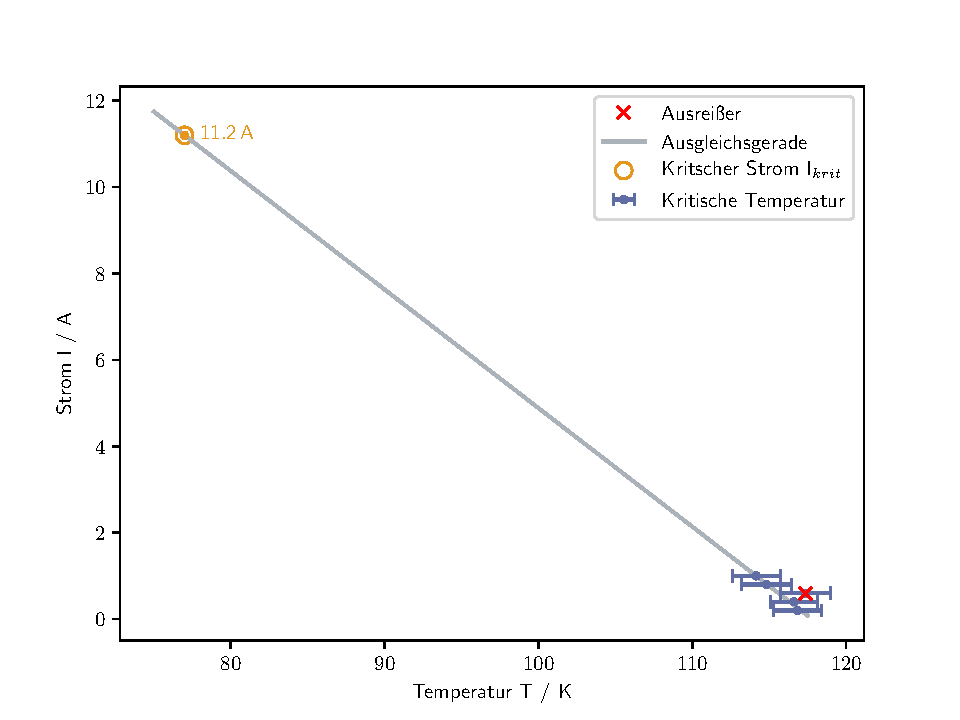
\includegraphics[width=0.8\textwidth]{Auswertung/I_krit_Pt/I_krit.pdf}
    \caption{Bestimmung der kritschen Stromstärke $I_{\text{c}}$ des SL \#1 Supraleiter ohne
		Magnet anhand einer 4-Punkt-Messung. Die kritschen Temperaturen $T^{\text{MCE}}_{\text{c}}$
		bei der dazugehörigen Stromstärke $I$ sind der Tabelle \ref{tab:Ic} zu entnehmen.
		Die gelbe Markierung kennzeichnet die Abschätzung des kritschen Stroms $I_{\text{c}}$
		und die rote Markierung kennzeichnet den aus der Auswertung unberücksichtigten Wert.}
\label{fig:Ic}
\end{figure}

\subsubsection{Mit Magnet}
\label{sec:mitB1}
Nun erfährt der SL \#1 Supraleiter eine Störung durch das starke Magnetfeld des
\#M3 Magnets. Wegen Messproblemen wird der kritsche Strom $I_{\text{c}}$ nur für zwei
Durchlaufstromstärken von $\SI{0,6}{\ampere}$ und $\SI{0,8}{\ampere}$ untersucht.
Dazu wird von jeder Messung
die kritsche Temperatur $T^{\text{MCE}}_{\text{c}}$ bei einem Widerstand von etwa
0,5-$\SI{0,6}{\ampere}$ abgelesen (siehe Anhang \ref{sec:AnhangTc}) und der
jeweilige Wert in Tabelle \ref{tab:Ic2} eingetragen.

\begin{table}
  \centering
  \caption{Kritsche Temperatur $T^{\text{MCE}}_{\text{c}}$ für fünf unterschiedliche
	Durchlaufstromstärken mit Magnetfeld des \#M3 Magnets.}
  \label{tab:Ic2}
  \sisetup{table-format=1.2}
  \begin{tabular}{S | S}
    \toprule
    {Stromstärke} & {kritsche Temperatur} \\
    {I / A} & {$T^{\text{MCE}}_{\text{c}}$ / K }  \\
    \midrule
		{0,6} & {107,33\pm3,51}	\\
		{0,8} & {104,00\pm2,85}	\\
    \bottomrule
  \end{tabular}
\end{table}

\noindent
Die kritsche Strom $I_{\text{c}}$ ergibt sich erneuert durch eine Extrapolation
bis $\SI{77}{\kelvin}$ mittels $\textit{Python 3.7.6}$, welche in Abbildung
\ref{fig:Ic2} dargestellt ist. Die Parameter der Ausgleichsgeraden
$I(T)=m\cdot T + b$ haben dabei folgende Werte:

\begin{equation*}
	m = \SI{-0.06}{\ampere\per\kelvin}
	\qquad
	b = \SI{7.05}{\ampere}
	\label{AF5}
\end{equation*}

\noindent
und der kritsche Strom $I_{\text{c}}$ damit einen Schätzwert von $\SI{2.42}{\ampere}$.

\begin{figure}[H]
    \centering
    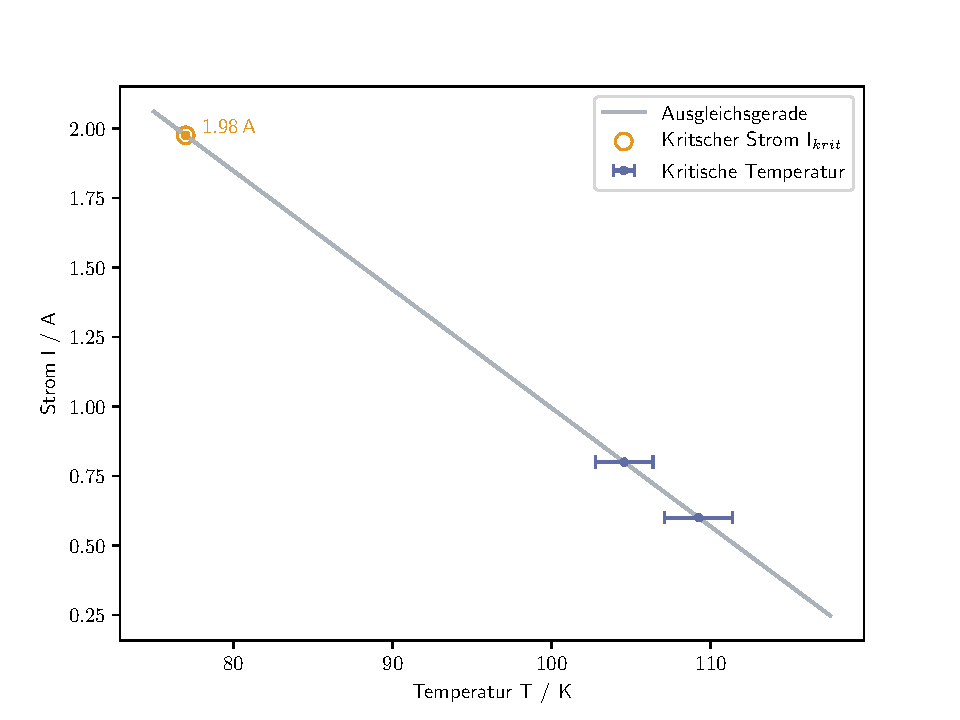
\includegraphics[width=0.8\textwidth]{Auswertung/I_krit_Pt_b/I_krit.pdf}
    \caption{Bestimmung der kritschen Stromstärke $I_{\text{c}}$ des SL \#1
		Supraleiter mit Störung durch den \#M3 Magnet anhand einer 4-Punkt-Messung.
		Die kritschen Temperaturen $T^{\text{MCE}}_{\text{c}}$
		bei der dazugehörigen Stromstärke $I$ sind der Tabelle \ref{tab:Ic} zu entnehmen.
		Die gelbe Markierung kennzeichnet die Abschätzung des kritschen Stroms $I_{\text{c}}$.}
\label{fig:Ic2}
\end{figure}

\subsection{Abschätzung des induzierten Stroms $I_{\text{ind}}$}
\label{sec:ind}
Zuletzt wird der mit dem \#M3 Magnenten induzierte Strom $I_{\text{ind}}$ am SL
\#4 Supraleiter-Ring abgeschätzt. Dazu misst die Hall-Sonde, in einem Abstand von
$z=0$ zum Mittelpunkt des Rings, ein induziertes Magnetfeld $B_{\text{ind}}$ von
$\SI{1,59}{\milli\tesla}$. Das Biot-Savart-Gesetz für kreisförmige Stromschleifen:

\begin{equation*}
	I_{\text{ind}}(z,R,B_{\text{ind}}) = \frac{2B_{\text{ind}}(z^2+R^2)^{3/2}}{\mu_0R^2}
\label{AF6}
\end{equation*}

\noindent
erlaubt es nun, den induzierten Strom $I_{\text{ind}}$ abschätzen, wobei der
Radius $R$ des SL \#4 Supraleiter-Ring $\SI{7,5}{\milli\meter}$ beträgt. Der
induzierte Strom lässt sich damit auf einen Wert von $\SI{18.98\pm0.51}{\ampere}$
abschätzen. Wegen einer möglichen nicht idealen Messposition in $z$-Richtung,
wird dem $I_{\text{ind}}$-Wert ein Fehler, welcher sich aus dem absoulte Fehler:
$|I_{\text{ind}}(z=0,R,B_{\text{ind}}) - I_{\text{ind}}(z=\SI{\pm0.1}{\milli\meter},R,B_{\text{ind}})|$
ergibt, zugeschrieben.
